\documentclass[11pt]{article}
\usepackage[T1]{fontenc}
\usepackage{times}%, babel}
\usepackage{secdot,natbib}
\usepackage{latexsym, amsthm, amsmath, amssymb, color, rotating, multirow, graphicx, hhline, array, tablefootnote}
\usepackage{scalefnt, enumerate}
\usepackage{footnote}
\usepackage{threeparttable,booktabs}
\usepackage{natbib}
\usepackage[hyphens]{url}
%\usepackage{bm, url}
%\usepackage{slashbox}
\usepackage{tikz,pgfplots}
%\usepackage{subcaption}
\usepackage[margin=10pt,font=small,labelfont=bf,labelsep=endash]{caption}
\usepackage{subfigure}
\usepackage{kotex} %Korean TeX
%\usepackage[latin9]{inputenc} % kotex package와 충돌. 향후 kotex 삭제하면 될 듯.




%%% ----------------------------------------------------------------------
%\clubpenalty=10000 \widowpenalty=10000
%\renewcommand{\baselinestretch}{1.5}
% \renewcommand{\theequation}{{\rm \thesection.\arabic{equation}}}
\renewcommand{\theequation}{{\rm \arabic{equation}}}
\oddsidemargin 0in  %.10in
\evensidemargin 0in
\hyphenpenalty 2000

\textwidth 6.5in    %6.5
\textheight 8.75in     %8.5
\topmargin 0.0in      %0in
\headsep 0in \makeatletter
\newcommand{\singlespacing}{\let\CS=\@currsize\renewcommand{\baselinestretch}{1.1}\tiny\CS}
\newcommand{\doublespacing}{\let\CS=\@currsize\renewcommand{\baselinestretch}{1.5}\tiny\CS}
\newcommand{\realdoublespacing}{\let\CS=\@currsize\renewcommand{\baselinestretch}{2.0}\tiny\CS}
\newcommand{\mydoublespacing}{\let\CS=\@currsize\renewcommand{\baselinestretch}{1.499}\tiny\CS}

\newtheorem{theorem}{Theorem}[section]
\newtheorem{proposition}[theorem]{Proposition}
\newtheorem{lemma}[theorem]{Lemma}
\newtheorem{corollary}[theorem]{Corollary}

\def\N{\mathbb{N}}
\def\1{\mathbf{1}}
\def\P{\mathbf{P}}
\def\E{\mathbf{E}}
\newcommand{\maximize}{\mathop{\mbox{{\rm maximize}}}\limits}
\newcommand{\minimize}{\mathop{\mbox{{\rm minimize}}}\limits}
\newcommand{\argmax}{\mathop{\mbox{{\rm arg\,max}}}\limits}


%\newcommand\ks[1]{{\textbf{#1}}}
\newcommand{\ks}[1]{{\color{blue} #1}}
\newcommand{\ju}[1]{{\color{magenta} #1}}
\newcommand{\yj}[1]{{\color{red} #1}}


\setlength\parindent{0cm}
\setlength{\parskip}{12pt}%

\renewcommand\ttdefault{cmvtt}

%%%%%%%%%%%%%%%%%%%%%%%%%%%%%%%%%%%%%%%%%%%%%%%%%%%%%%%%%%%%
\begin{document}

\begin{center}
{{\Large \bf Response to Review Reports on POM-Jul-20-SI-0934.R1}\\[6mm]
{\LARGE ``Sharing Economy in the Cloud:\\ Pricing Schemes for Peer-to-Peer Storage Platforms''}\\[15mm]}
\end{center}

\baselineskip 18pt

\noindent \underline{\large \bf General Response to the Review Team}

We sincerely appreciate the review team for the opportunity to further improve our paper. The review team has provided valuable comments and suggestions on our revised manuscript in the last round. %We believe that the concerns raised in this round are valid and informative to clarify our contributions, improve the validity of our model and results, and streamline related literature.

In this revision, we have exerted our best efforts to address all points you raised. We have first outlined and summarized our major revisions made in this round. Then, we have provided detailed point-to-point responses to the comments raised by Senior Editor and each of the two
referees. 
We hope that the review team finds our revision meets the expected quality.

\textbf{\large 1. Integrating Algorithmic Decisions into the Main Model}\\
Related to: \textbf{[SE Point 1] [R1 Point 2] [R2 Point A1]}

We have incorporated endogenous algorithmic decisions into our model and strengthened our originality. Specifically, the review team raised a concern about the uniqueness of P2P storage sharing and our model. Relatedly, we suggested the algorithmic decision as a unique feature of our analysis, but the main model did not include this aspect and postulated an exogenous algorithm.

In this revision, we have revamped our main model by integrating an endogenous redundancy algorithm (\textbf{Theorem 1} in the new version). As shown in \textbf{General Response Figure 1}, we have supposed that the P2P storage platform first decides its redundancy algorithm. After that, the market size of peers (i.e., $n_r$ and $n_p$) is realized, and the platform responds to this market environment by making the pricing decision $(p_s, p_b)$.

\setcounter{figure}{0}
\begin{figure}[ht!]
\def\figurename{General Response Figure}
\centering
\includegraphics[width=16cm]{fig1_timeline_revised.pdf} 
\caption{The Sequence of Events}
\end{figure}

We have found that the platform always needs to set the algorithm that minimizes the total operating costs of providers in the P2P network. This is intuitive considering that a lowered operating cost implies that the P2P network becomes more efficient and attractive to potential providers. Importantly, this result is identical across all pricing schemes, allowing us to maintain the existing lemmas and theorems.

\textbf{\large 2. Examining the Validity of the Findings}

\textbf{2.1. Additional Heterogeneity Dimensions}\\
Related to: \textbf{[SE Point 2a] [R2 Point A2a] [R2 Point A2b] [R2 Point A4a] [R2 Point A4b]}

The review team suggested additional possibilities of the renter/provider heterogeneity, which provided valuable directions to further convince our results. However, it is worth noting that our main model already accounts for three important sources of heterogeneity—two dimensions of renter heterogeneity (download frequency, utility per download) and one dimension of provider heterogeneity (operating costs). Therefore, we have maintained and justified the current model's peer heterogeneity and discussed the potential consequences of additional  possibilities.

To further validate our findings, we have also conducted several numerical analyses. Specifically, we have examined various scenarios on renters' storage volume, bandwidth volume, and utility per unit bandwidth volume. The results show that our findings remain consistent across all heterogeneity sources and scenarios we have considered.

\textbf{2.2. Is the Redundancy Rate Achievable?}\\
Related to: \textbf{[SE Point 2c] [R1 Point 1]}

% [Previous Paragraph]
% Our model has already accounted for the effects of pricing on the provider and renter decisions, and importantly, the realized redundancy ratio $m/k$ is not affected by how many renters/providers are willing to join the platform. Specifically, the platform does not assign renters to individual providers beyond its storage capacity in our model. That is, the required redundancy is achieved because the platform cannot serve the excessive storage demand. We have added more detailed explanations to the new manuscript to clarify the redundancy algorithm.

% [Revised Paragraph (1/2)]
Our model has already accounted for the effects of pricing on the provider and renter decisions, and we summarize its implications related to the realized redundancy ratio in this response letter. Basically, for each contract, the platform sets the profit-maximizing redundancy rate $m/k$ and assigns providers and renters proportionally to $m/k$. Then, automatically, any storage supply (demand) not assigned to this contract is idle (rationed). In other words, the realized redundancy ratio depends only on the predetermined $m/k$, not $n_r$ and $n_p$.

% [Revised Paragraph (2/2)]
In this regard, pricing can play a profit-enhancing role, not managing the redundancy rate. When there is an excessive demand compared to the storage capacity, the platform can improve its profit by raising service fees and discouraging renters with a lower willingness to pay until participating providers can serve all renters willing to pay for the prices. Again, this affects the supply-demand ratio, but not the redundancy rate of assigned storage. We have added more detailed explanations to the new manuscript to clarify the redundancy algorithm.

Thankfully, we could learn from this point that some of our previous solutions are not optimal under substantially low $\xi$ (i.e., operating cost). Our previous analysis did not consider that $n_p$ is the upper limit of the number of participating providers. For the cases with sufficient operating costs, which is our main interest, this does not change our results. However, if $\xi$ is very low and then all providers join the platform under the previously suggested pricing, we have found that this might alter the optimal service fees in some conditions. However, these conditions are very unlikely to occur in practice because the profitability and operating costs are major concerns in online forums for P2P storage platforms.

\textbf{2.3. Information Sources}\\
Related to: \textbf{[SE Point 2b] [R2 Point A3]}

There are various sources offering \textit{a priori} information, which helps potential providers make rational expectations before joining the platform. For example, SiaStats is a website that publicizes Sia's storage sharing status, such as used storage, number of transactions, network revenues, and hash rates. Also, individual providers have actively analyzed and shared their profitability in online forums, such as Reddit. Moreover, the P2P platforms publicly notice the minimum requirement and recommended computing capacity. Such information also partially informs them about their operational costs in the future.

When providers are operating in the network, they can receive real-time feedback on their network performance. Hence, they can quickly correct their behaviors on the platform. Furthermore, even when unsuccessful on the platform, they can immediately leave the network with some financial loss as they can do in other digital markets. Considering the platform-offered information, online forums, and easiness of market entry/exit, we expect that P2P participants will reach market equilibrium very rapidly. We have described this background in the revised version.

\textbf{\large 3. Restructuring and Clarifying the Paper Flow}\\
Related to: \textbf{[SE Point 3] [R2 Point B1] [R2 Point B1a] [R2 Point B1b] [R2 Point B2]}

We have restructured our subsections to inform readers about notations better. Specifically, we have moved our notations and equations of renter behaviors to the beginning of Section 3.2, helping readers understand volume notations used in provider decisions. Moreover, we have revised our description of equations in Sections 3 and 4.

In addition, we have reorganized the literature review section and provided a separate section on our contributions to the literature. Along with integrating algorithmic decisions into the main model, our reorganization helps streamline the literature and emphasize our originality. We have summarized the structure of this revised version in comparison to the structure of the last version in \textbf{General Response Table 1}.\\

%\newpage
\begin{table}[ht!]\footnotesize 
\def\tablename{General Response Table}
\caption{Paper Structure before and after This Revision}
\begin{center}
\begin{tabular}{p{0.5\linewidth} | p{0.5\linewidth}}
\toprule
\textbf{Before Revision} & \textbf{After Revision} \\ \hline

\textbf{1. Introduction} & \textbf{1. Introduction}\\ \\

\textbf{2. Related Literature} & \textbf{2. Related Literature}\\
&\multirow{4}{*}{\begin{tabular}[c]{@{}l@{}}
\hspace{2mm} 2.1. Pricing and Capacity Management in Centralized Cloud\\ 
\hspace{2mm} 2.2. P2P Sharing of Computing Resources\\ 
\hspace{2mm} 2.3. Sharing Economy and Online Platforms  \\
\hspace{2mm} 2.4. Contributes to the Literature \end{tabular}}\\
\\
\\
\\
\\
\textbf{3. Model} & \textbf{3. Model}\\ 
\multirow{2}{*}{\begin{tabular}[c]{@{}l@{}}
\hspace{2mm} 3.1. Model Setups\\ 
\hspace{2mm} 3.2. Decisions of Providers and the Platform
\end{tabular}}
&
\multirow{5}{*}{\begin{tabular}[c]{@{}l@{}}
\hspace{2mm} 3.1. Model Setups\\ 
\hspace{2mm} 3.2. Peer Decisions\\
\hspace{4mm} 3.2.1. A Renter’s Decision\\
\hspace{4mm} 3.2.2. A Provider’s Decision\\
\hspace{6mm} \textbf{\textit{Lemma 1}} (Providers’ decisions)
\end{tabular}}\\
\\
\\
\\
\\
\\
\textbf{4. Analysis of First-Best Prices} & \textbf{4. Optimal Decisions}\\
\multirow{5}{*}{\begin{tabular}[c]{@{}l@{}}
\hspace{2mm} 4.1. Optimal Service Fees for Each Pricing Scheme\\ 
\hspace{4mm} \textbf{\textit{Lemma 1}} (First-best prices)\\
\hspace{2mm} 4.2. Platform's Profit and System Surplus\\
\hspace{4mm} \textbf{\textit{Theorem 1}} (Comparison of profit and total surplus under
\\
\hspace{6mm} first-best prices)\\
\\
\\
\\
\\
\end{tabular}}
&
\multirow{7}{*}{\begin{tabular}[c]{@{}l@{}}
\hspace{2mm} 4.1. Optimal Service Fees\\ 
\hspace{4mm} 4.1.1. First-best Prices  \\
\hspace{6mm} \textbf{\textit{Lemma 2}} (First-best prices)\\
 \hspace{4mm} 4.1.2. Market-clearing Prices\\
 \hspace{6mm} \textbf{\textit{Lemma 3}} (Market-clearing price thresholds)\\
\hspace{2mm} 4.2. Optimal Redundancy Algorithm\\
\hspace{4mm} \textbf{\textit{Theorem 1}} (Optimal redundancy algorithm)
\end{tabular}}
\\
\\
\\
\\
\\
\\
\\
\\
\textbf{5. Analysis of Market-Clearing Prices } & \textbf{5. Pricing Schemes, Profit, and System Surplus}\\ 
\multirow{3}{*}{\begin{tabular}[c]{@{}l@{}}
\hspace{2mm} \textbf{\textit{Lemma 2}} (Market-clearing price thresholds)\\ 
\hspace{2mm} \textbf{\textit{Theorem 2}} (Comparison of profit and total surplus \\
\hspace{4mm} under market-clearing prices)\\
\\
\\
\\
\\
\\
\end{tabular}}
&
\multirow{7}{*}{\begin{tabular}[c]{@{}l@{}}
\hspace{2mm} 5.1. Under First-Best Prices\\ 
\hspace{4mm} \textbf{\textit{Theorem 2}} (Comparison of profit and total surplus \\
\hspace{6mm} under first-best prices)\\
\hspace{2mm} 5.2. Under Market-Clearing Prices\\
\hspace{4mm} \textbf{\textit{Theorem 3}} (Comparison of profit and total surplus under \\
\hspace{8mm} market-clearing prices)\\
\\
\\
\end{tabular}}\\
\\
\\
\\
\\
\\
\\
\textbf{6. Analysis of Platform’s Endogenous Operations Decisions} & \textbf{6. Model Extension and Discussion}\\ 
\multirow{7}{*}{\begin{tabular}[c]{@{}l@{}}
\hspace{2mm} 6.1. The Platform’s Endogenous Decision \\
\hspace{6mm} on Redundancy Algorithms\\ 
\hspace{4mm} \textbf{\textit{Theorem 3}} (Comparison of profit and total surplus under\\
\hspace{6mm} endogenous algorithm) \\
\hspace{2mm} 6.2. The Platform’s Endogenous Decision on Commission Rates\\
\hspace{4mm} \textbf{\textit{Theorem 4}} (Comparison of profit and total surplus \\
\hspace{8mm} under endogenous commission rates)\\
\\
\\
\\
\\
\end{tabular}}
&
\multirow{6}{*}{\begin{tabular}[c]{@{}l@{}}
\hspace{2mm}6.1. Endogenous Decision on Commission Rates\\ 
\hspace{4mm} \textbf{\textit{Theorem 4}} (Comparison of profit and total surplus under \\
\hspace{6mm}endogenous commission rates under market-clearing prices)\\
\hspace{2mm} 6.2. Discussion on Assumptions\\
\hspace{4mm} 6.2.1. Assumptions on Providers\\
\hspace{4mm} 6.2.2. Assumptions on Renters\\ 
\\
\\
\\
\\
\\
\end{tabular}}\\
\\
\\
\\
\\
\\
\\
\\
\textbf{7. Discussion and Conclusion} & \textbf{7. Conclusions}\\ 
\bottomrule
\end{tabular}
\end{center}
\end{table}

\newpage

%%%%%%%%%%%%%%%%%%%%%%%%%%%%%%%%%%%

\noindent \underline{\large \bf Authors' Response to SENIOR EDITOR}\\[-11mm]

%%%%%%%%%%%%%%%%%%%%%%%%%%%%%%%%%%%
\begin{quotation}
{\em
\noindent \textbf{Senior Editor: } I sent the revised paper to the same review team. While they acknowledge and appreciate the effort exerted by the authors, both reviewers continue to have major concerns with the paper. As a result, both reviewers suggest another round of “major revision.” I went over the revised paper and the reviewers’ comments, and I concur with the reviewers’ comments. I would like to recommend another “major revision” and give the authors the opportunity to address the concerns. 
 
Given the reviewers’ expertise and the thorough reports they provide, I have little to add. Rather, I would refer the authors to the detailed comments in the reviewers’ reports. Next, I would like to highlight three major concerns. 
}
\end{quotation} \vspace{-4mm}

We thank you for your valuable comments. The feedback in this round allowed us to substantially improve several aspects of the study, including the model's clarity, robustness, uniqueness, and literature flow. We have devoted considerable efforts to address the issues raised by the review team satisfactorily and provided our point-by-point responses to the review team's concerns in the succeeding paragraphs. We hope that our efforts meet your expectations.

%%%%%%%%%%%%%%%%%%%%%%%%%%%%%%%%%%%


%%%%%%%%%%%%%%%%%%%%%%%%%%%%%%%%%%%%%%%%%%%%%%%%%%%%%%%%%%%%%%%%%%%%%%%%%
\noindent\textbf{Main Concern: Uniqueness of Storage Sharing}\\[-11mm]
%%%%%%%%%%%%%%%%%%%%%%%%%%%%%%%%%%%%%%%%%%%%%%%%%%%%%%%%%%%%%%%%%%%%%%%%%

\begin{quotation}
{\em
\noindent \textbf{Senior Editor (Point 1): }  
As R2 correctly notes, it remains unclear in this revised version what are the unique features of storage sharing (compared with other peer-to-peer platforms) and whether these unique features are captured by the main model. If this study is positioned to focus on storage sharing, the authors may want to elaborate on its distinct features, ensure the model captures some (if not all) of these features, and explain how these distinct features connect with the main results. Of course, the alternative is to position the paper to study peer-to-peer platforms in general. In that case, it will be fine to assume away some specifics of a particular type of platforms. In either way, the authors should be upfront and present clearly about that to readers, and articulate the contribution beyond the existing literature. 
}
\end{quotation} \vspace{-4mm}

We have decided to focus on storage sharing and elaborate how distinct our setup and implications are from other peer-to-peer platforms. As noted by Reviewer 2's \textbf{Point A1}, pricing schemes and renter/provider (buyer/supplier) heterogeneity are common features of P2P platforms. Also, our previous model accounts for the algorithm decision only in its extension part.

In this revision, we have strengthened our main model and its description to emphasize our distinct model  setup differentiated from other P2P contexts. First, we have relaxed the main model's assumption that the redundancy algorithm is exogenously given. We have incorporated this decision and let the platform choose the algorithm $(\theta, t)$ to maximize its expected profit (see our new \textbf{Theorem 1}).

Second, we have further elaborated on how our provider's cost structure differs from other P2P contexts. Specifically, our model allows providers' operating costs to be affected by renters’ usage levels, contrary to typical model settings in the sharing economy literature. This enables us to better reflect providers' operational burden and corresponding in-out decisions.

Please refer to our responses to Reviewer 2's \textbf{Point A1} for more details.

%%%%%%%%%%%%%%%%%%%%%%%%%%%%%%%%%%%%%%%%%%%%%%%%%%%%%%%%%%%%%%%%%%%%%%%%
\noindent\textbf{Main Concern: Model}\\[-11mm]
%%%%%%%%%%%%%%%%%%%%%%%%%%%%%%%%%%%%%%%%%%%%%%%%%%%%%%%%%%%%%%%%%%%%%%%%%

\begin{quotation}
{\em
\noindent \textbf{Senior Editor (Point 2a): } Both reviewers continue to have concerns with the model setup. 
(a) Heterogeneity of users: As R2 points out, users (both renters and providers) can be heterogeneous in other dimensions as well, which is a good observation. The authors are encouraged to explore possible models which consider heterogeneity in multiple dimensions. However, I would think that the review team will also be fine if the authors can only incorporate some heterogeneity into the model (e.g., the heterogeneity the current model considers). If they take this approach, the authors should elaborate on at least the following two aspects---why the authors consider this specific heterogeneity against other possible heterogeneity, and how the chosen model setup (i.e., ignoring the other possible heterogeneity) affects the main insights.  }
\end{quotation} \vspace{-4mm}

We sincerely appreciate the review team's constructive comments on various dimensions of heterogeneity. Considering that our main model already accounts for three important sources of heterogeneity---two dimensions of renter heterogeneity (download frequency, utility per download) and one dimension of provider heterogeneity (operating costs), we have decided to adopt the second approach, which maintains and justifies the current model's user heterogeneity and investigates with the discussion on the consequences of other heterogeneity. In addition, we have shown that our findings remain consistent even when such additional heterogeneity is considered by conducting numerical analyses. Below, we have summarized how we have addressed each point in this revision.

\textbf{Heterogeneity of Renter's Storage Volume.} Reviewer 2's \textbf{Point A2a} suggested that renters' storage volumes are substantially heterogeneous, leading to various renter segments---e.g., renters with large storage volume and low frequency download request, and those with small storage volume and highly frequent download request. We admit that ignoring this heterogeneity is a big missing point, and thus, we need to understand its potential consequences. We have addressed this point by conducting a numerical analysis that incorporates such renter segments. The results suggest that the main insights from the basic setup remain unchanged under several conditions where various segments coexist in the market. Please refer to our responses to Reviewer 2's \textbf{Point A2a} for the technical details.

\textbf{Heterogeneity of Renters' Bandwidth Volume.} Our model already accounted for the heterogeneous download frequency and utility per volume. In this revision, we have numerically tested whether our findings remain consistent when we consider an additional dimension or an alternative functional form of heterogeneity. As noted by Reviewer 2's \textbf{Point A4a}, the independence assumption between a renter's bandwidth utility and her download frequency may not hold in practice. We have numerically analyzed the consequences of assuming a positive correlation between utility per download and download frequency and obtained consistent results. Also, Reviewer 2's \textbf{Point A4b} pointed out that the current parametric assumption may drive our findings. Hence, we have conducted a numerical study on whether other functional forms of download frequency yield the same or different insights. By testing other parameter values of the Pareto distribution ($b$), which manipulate the proportion of high-frequency renters, we have obtained qualitatively consistent results across all tested scenarios. 

\textbf{Heterogeneity of Provider's Storage Volume.} Reviewer 2's \textbf{Point A2b} indicated that the assumption that each provider supplies a unit volume of unused capacity requires a condition: the provider's income and cost are both proportional to the volume of the capacity provided. Accordingly, we have provided this assumption's specific justification and potential consequences when this assumption does not hold. To summarize, our assumption is plausible for the following reasons. First, several sources of operating costs are proportional to bandwidth usage, e.g., bandwidth and electricity costs. Second, bandwidth usage is likely proportional to storage volume because P2P storage platforms tend to assign more contracts to high-volume providers. Please refer to our responses to Reviewer 2's \textbf{Point A2b} and the revised manuscript for more details. 

%%%%%%%%%%%%%%%%%%%%%%%%%%%%%%%%%%%%%%%%%%%%%%%%%%%%%%%%%

\begin{quotation}
{\em
\noindent \textbf{Senior Editor (Point 2b): } (b) Information: R2 raises a question about how an individual provider could learn the information about the expected demand, which requires some clarification. If there is no specific mechanism or channel for providers to learn this information, I wonder if their “rational expectation” works. At any rate, the authors should carefully think about this and clearly explain how providers know the expected demand. 
}
\end{quotation}\vspace{-4mm}

\newpage
This is a valid concern that providers' rational expectation requires \textit{a priori} information and relevant sources. Following the review team's comments, we have carefully investigated how P2P storage providers obtain information before joining the platform. We have found that P2P storage platforms and online forums offer valuable information to potential providers.\footnote{Some examples of information sources:
\begin{itemize}
    \item SiaStats: \url{https://siastats.info/}
    \item Reddit community for Sia \url{https://www.reddit.com/r/siacoin/}
    \item Storj's prerequisites: \url{https://docs.storj.io/node/before-you-begin/prerequisites/}
    \item Filefox (a Filecoin blockchain explorer): \url{https://filfox.info/en/}.
\end{itemize}} 
For instance, SiaStats publicizes Sia's storage sharing status, such as used storage, number of transactions, network revenues, and hash rates. Also, P2P platforms notice their minimum requirement and recommended capacity of computing resources in advance, which can partially inform providers about their expected operating costs. Furthermore, individual providers have actively analyzed and shared their profitability in online forums like Reddit, allowing following providers to make more informed decisions.

After participating in the networks, providers can receive real-time feedback on their network performance; thus, they can quickly correct their behaviors on the platform. Even when unsuccessful on the platform, they can quickly leave the network similarly to other digital markets. Due to the platform-offered information, online forums, and easiness of market entry/exit, we expect that P2P participants will reach market equilibrium very rapidly.

We further describe how we have addressed this issue in our response to R2's \textbf{Point A3}.

\begin{quotation}
{\em
\noindent \textbf{Senior Editor (Point 2c): }
(c) Probability of Service Failure: R1 correctly notes that is it is not rigorous to claim that “by setting a proper $m$ and $k$, the chance of service failure is very small,” because price is endogenous and it affects the number of active providers. The authors should at least examine whether the desirable m and k will occur in equilibrium (under the equilibrium price). 
}
\end{quotation}\vspace{-4mm}

We thank you for this insightful comment and regret insufficiently elaborating how P2P storage platforms and our model work. As you noted by Reviewer 1's \textbf{Point 1}, prices do affect the number of participating providers and the platform’s total storage capacity. Our model has already accounted for this aspect, and notably, the realized redundancy ratio $m/k$ is not affected by how many renters/providers are willing to join the platform. To be specific, the platform does not assign renters to individual providers beyond its storage capacity in our model. That is, the required redundancy is achieved because the platform cannot serve the excessive storage demand. Of course, this situation deviates from the profit maximization because the platform can improve its profit by raising service fees and discouraging renters with a lower willingness to pay. In anyways, regardless of how many renters are not served, the redundancy ratio $m/k$ holds due to the provider-renter contract structure.

In addition, thanks to R1's comments, we have reexamined whether and when our previous solutions of service fees remain optimal under the given algorithm parameters $m$ and $k$. We have found that some of our previous solutions are not optimal under substantially low $\xi$ (i.e., operating cost). Our previous version missed the point that $n_p$ works as the upper limit of the number of participating providers. When operating costs are sufficiently high, which is our primary interest, this limit does not affect our results. However, when $\xi$ is very low, and then all providers participate in the platform under the previously suggested pricing, we have found that the upper limit might affect the optimal service fees in some conditions.

% because the platform needs to crowd out some renters by raising prices to maximize its profit. 

However, these conditions are very unlikely to occur in practice because the profitability and operating costs are major concerns in online forums for P2P storage platforms.\footnote{The profitability and operating costs are widely discussed among Storj's official forum (https://forum.storj.io/) and other forum users (e.g., Reddit).} Hence, we do not consider such cases in our main analysis and separately provide their results in Appendix C.

For more details, please see our responses to Reviewer 2's \textbf{Point 1}.\\

%%%%%%%%%%%%%%%%%%%%%%%%%%%%%%%%%%%%%%%%%%%%%%%%%%%%%%%%%%%%%%%%%%%%%%%%
\noindent\textbf{Main Concern: Writing}\\[-11mm]
%%%%%%%%%%%%%%%%%%%%%%%%%%%%%%%%%%%%%%%%%%%%%%%%%%%%%%%%%%%%%%%%%%%%%%%%%

\begin{quotation}
{\em
\noindent \textbf{Senior Editor (Point 3): } I agree with R2 that the writing could be further improved. The reviewer generously provides detailed suggestions. I would encourage the authors to follow the suggestions and go even beyond to further polish the paper. }
\end{quotation} \vspace{-4mm}

We appreciate the review team for providing great suggestions on our writing, which enabled us to better polish our manuscript. Following Reviewer 2's \textbf{Points B1 and B1a}, we have restructured our subsections to better inform readers about notations. Specifically, we have moved our notations and equations of renter behaviors to the beginning of Section 3.2, helping readers understand volume notations used in provider decisions. Moreover, we have revised our description on $\hat{\omega}_b$ and $V_{bp}$ in Sections 3 and 4.

Regarding the literature review, we have followed Reviewer 2's comments in \textbf{Point B2}. We have reorganized the literature review section and provided a separate section on our contributions to the literature. Combining with our efforts to clarify the uniqueness of storage sharing, we could better streamline the literature and emphasize our originality.

%%%%%%%%%%%%%%%%%%%%%%%%%%%%%%%%%%%%%%%%%%%%%%%%%%%%%%%%%

\begin{quotation}
{\em
\noindent \textbf{Senior Editor: } I am very thankful to the two experienced reviewers for providing their valuable comments. I hope the authors can take advantage of their comments and further improve the paper. The authors did a good job clarifying many issues in the first round. I would encourage the authors to address the reviewers’ comments with the same standard. Good luck with the revision. }
\end{quotation}\vspace{-4mm}

We are so grateful to the review team for providing constructive directions to improve our analysis and contributions. We hope our efforts to address all concerns raised in the previous round meet your expectation.

\newpage
%%%%%%%%%%%%%%%%%%%%%%%%%%%%%%%%%%%%%%%%%%%%%%%%%%%%%%%%%%%%%%%
\noindent \underline{\large \bf Authors' Response to Reviewer 1}
%%%%%%%%%%%%%%%%%%%%%%%%%%%%%%%%%%%%%%%%%%%%%%%%%%%%%%%%%%%%%%%


%%%%%%%%%%%%%%%%%%%%%%%%%%%%%%%%%%%%
\begin{quotation}
{\em
\noindent \textbf{Reviewer 1 (Point 1): }
The revised manuscript addressed part of my concerns, while the following two major concerns are still not addressed: 

1. About the probability of service failure. The revised paper argues that by setting a proper $m$ and $k$, the chance of service failure is very small. Essentially, this is based on that the required $m$ and $k$ can always be achievable, regardless of price. However, it is not the case since price will certainly affect the number of active providers, which will affect the achievable $m$.   
 
The fact that the platform penalizes the providers who do not maintain certain uptime does NOT mean that the redundancy level can be achieved since it also largely depends on price, which is the decision to be made. 
 
All in all, this is still a big missing point and incorrect assumption. 
}
\end{quotation}\vspace{-4mm}

We sincerely thank you for this constructive comment. As you noted, prices affect the number of participating providers and the platform's total storage capacity, but it is not related to \textit{realized} redundancy rates for the following reasons.
%Therefore, for some pricing schemes and service fees, the storage demand of renters willing to use the service (i.e., $\theta \upsilon_s$) can be higher than the storage supply by participating providers (i.e., $\omega_s$). However, even in such cases, the ratio $m/k$ always holds because renters beyond the capacity are not assigned to individual providers. In other words, the required redundancy is always achieved because the platform cannot serve the excessive storage demand. 
The platform assigns a designated number of providers and renters for each contract following the redundancy rate of $m/k$. If the platform increases the rate, it needs more providers to serve one renter. However, even in this case, the ratio $m/k$ does not change because any excessive storage demand not assigned to the contract becomes rationed. In other words, the required redundancy is always achieved regardless of $n_r$ and $n_p$. While not affecting the realized redundancy, pricing helps better manage the excessive demand. Specifically, the platform can improve its profit by raising service fees and discouraging renters with a lower willingness to pay. It can increase service fees until participating providers can serve all renters willing to pay for the prices. Again, regardless of how many renters are not served, the redundancy ratio $m/k$ holds due to the provider-renter contract structure.

Although our model has already reflected this aspect, we admit that the previous manuscript did not sufficiently explain how our model works and what the redundancy constraint means. Therefore, in the revised manuscript, we have added these details as follows:

``We consider a profit-seeking platform that gathers renters and providers in the common marketplace and enables encrypted contracts for storage sharing services between them. The P2P storage platform first sets the redundancy rate $\theta$ and the required uptime $t$. For a given $\theta$, the platform can assign renters to providers until the storage demand multiplied by $\theta$ reaches the total storage capacity.'' (page 13)

``(...) In this equation, $\min\{\theta \upsilon_s, \omega_s\}$ implies the total volume of shared storage. Specifically, when there are sufficient participating providers, all renters can store their files in the network. Thus, $\theta \upsilon_s$ is identical to the total stored volume. In contrast, when the storage capacity of participating providers is insufficient to meet the demand, the platform can serve storage up to $\omega_s$. In this case, the platform serves the renter's demand until $\omega_s / \theta$, which is the total storage capacity divided by the redundancy ratio.'' (page 17)

% 1) 어떤 pricing 내에서 실제로 renter가 provider보다 더 많을 수 있음($\theta$고려). 이 경우에는 이 redundancy rates가 achievable하지 않게 보일 수도 있음.\\
% 2) 그런데 사실 이 경우에도 이 $m/k$는 성립하는 것임. 왜냐하면 그냥 일부 renter가 저장을 못하는 것일 뿐.\\
% 3) 하지만 이 경우에 기업은 profit을 최대화하는 관점에서는 price를 높임으로써 renter들을 이탈시키고, provider에 대해 더 많은 incentive를 제공하는 형태로 이 renter 및 provider 사이의 interaction을 pricing을 통하여 이용할 수 있음\\
% 4) 결과적으로 모든 renter가 저장을 하면서 $m/k$도 성립하는 형태로 pricing을 할 수 있게 됌.\\

% i) failure rate를 만족하는 redundancy rate가 존재하느냐 \\
% ii) 그러면 위 redundancy rate대로 renter / provider 사이에서 할 수 있느냐\\

Also, thanks to your comments, we have revisited whether and when our previous solutions of service fees remain optimal under the given algorithm parameters $m$ and $k$. We have revealed that some of our previous solutions are not optimal under substantially low $\xi$ (i.e., operating cost) due to the following reasons. 
% because the platform needs to crowd out some renters by raising prices to maximize its profit.
Previously, our solutions did not consider that $n_p$ is the upper limit of the number of participating providers. We have found that when operating costs are not negligible to potential providers, this does not change our results. However, if $\xi$ is very low and then all providers join the platform under our previous solution, we have found that this might alter the optimal service fees in some conditions. Specifically, lower operating costs are more advantageous for providers, but they cannot affect the total capacity when $n_p$ providers have already joined the platform. We have taken account of this constraint in our revised analysis and identified the conditions where the optimal service fees should deviate from our previous solutions to meet the given redundancy level.

Let us note in advance that these conditions are very unlikely to occur in practice. To be specific, the upper limit $n_p$ matters when operating costs are so small (i.e., small $\xi$) that all potential providers would join the platform under either the current $\xi$. Contrary to such conditions, we have observed that the profitability and operating costs are major concerns in online forums for P2P storage platforms.\footnote{The profitability and operating costs are widely discussed among Storj's official forum (https://forum.storj.io/) and other forum users (e.g., Reddit).} As a result, many potential providers hesitate to offer their storage and bandwidth services. For this reason, we do not consider such cases in our main analysis and separately provide their results as below.

% \textbf{When are previous solutions not optimal?} 

% We have identified the conditions where our previous solutions are optimal or not as follows:

% \textit{Case }1) when $\frac{3}{4}\alpha \le \xi$, our all previous solutions for all pricing schemes are optimal,\\
% \textit{Case }2) when $\frac{3}{10}\alpha \le \xi < \frac{3}{4}\alpha$, some of our previous solutions for some pricing schemes cannot be optimal,\\
% \textit{Case }3) when $\xi < \frac{3}{10}\alpha$, all of our previous solutions are not optimal.

% In sum, our previous solutions are optimal only when $\frac{3}{4}\alph a \le \xi$ (\textit{Case }1). Below, we have discussed the implications of our findings when the previous solutions are not optimal.

% Note that we can generalize this condition as $\frac{2b-1}{2b}\alpha \le \xi$ for all $b$. We have provided the proof of these cases in the Appendix of this response letter.

\textbf{What are the outcomes where the previous solutions are not optimal?} We have found that our previous solutions are optimal only when $\frac{3}{4}\alpha \le \xi$. Below, we have discussed the implications of our findings when the previous solutions are not optimal.

We conduct a numerical analysis 
% for \textit{Case }2 and d \textit{Case }3,
for extremely low $\xi$, where our previous solutions may not optimize the profits of some pricing scheme. We have found that as $\xi$ decreases (i.e., operating costs decrease), the two-part tariff and the hybrid pricing can be less effective in boosting the total surplus than the subscription-based pricing for the following reasons.

Since providers do not respond to bandwidth fees sensitively under small $\xi$, raising prices does not help renters find more capacity while it increases their financial burden. Therefore, the two-part tariff, which compensates for providers' bandwidth services, becomes less effective in boosting system surplus than the subscription-based pricing. Consequently, the surplus implication of pricing schemes is similar to the first-best prices under substantially small $\xi$. The small $\xi$ affects the surplus implication of the hybrid pricing similarly, as shown in our numerical analysis (\textbf{Figure R1-1}). The graph presents the relative system surplus of the two-part tariff and hybrid pricing under $\xi = 0.2$, $\theta=3$, $b=2$, $\lambda_0=1$, $q=2$, and $\alpha=0.95$, where $\xi$ is sufficiently smaller than $\frac{3}{4}\alpha$. The results demonstrate that the subscription-based pricing outperforms these schemes in any small $\xi$ in this case.

% When $\xi$ is substantially small (i.e., low operating costs), all potential providers are willing to share their storage and participate in the platform. In this situation, the platform can improve its profit by adjusting prices until the participating providers' capacity meets the storage demand, indicating that the current prices are not optimal.

\setcounter{figure}{0}
\begin{figure}[ht!]
\centering
\def\figurename{Figure R1 -}
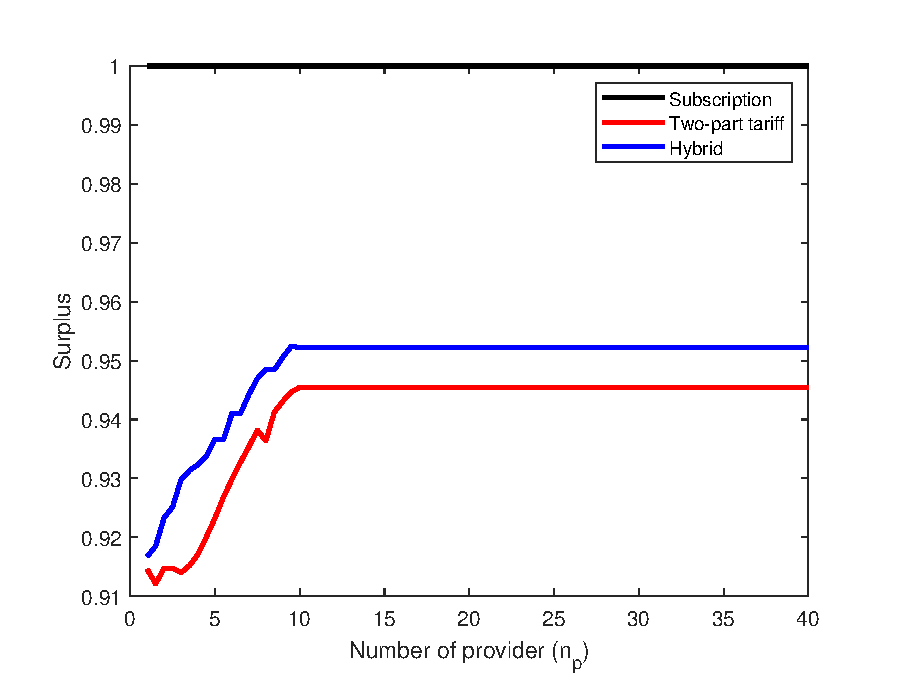
\includegraphics[width=8cm]{figure_3rd_final/f_low.eps} 
\caption{Surplus Comparison for Extremely Low Operating Costs}
\end{figure}

In the revised manuscript, we have discussed this issue as follows:

``First, our model excludes the case where operating costs are negligible for potential providers; that is, we assume that $\xi > \frac{3}{4} \alpha$. Although online forums for P2P storage platforms have been significantly concerned the profitability and operating costs, it is still insightful to understand the consequences of pricing schemes when operating costs become negligible. In Appendix C, we provide technical details of a numerical study examining how small operating costs (i.e., $\xi \le \frac{3}{4} \alpha$) can affect our results. Below, we summarize key insights from this analysis.

When $\xi$ is substantially small (i.e., low operating costs), all potential providers are willing to share their storage and participate in the platform. Since providers do not respond to bandwidth fees sensitively under small $\xi$, raising prices does not help renters find more capacity while it increases their financial burden. Therefore, the two-part tariff and the hybrid pricing, which compensate for providers' bandwidth services, are less effective in boosting system surplus than the subscription-based pricing. Consequently, the surplus implication of pricing schemes is similar to the first-best prices under substantially small $\xi$.'' (pages 30-31)

%%%%%%%%%%%%%%%%%%%%%%%%%%%%%%%%%%%%

\begin{quotation}
{\em
\noindent \textbf{Reviewer 1 (Point 2): } 2.    Same for assumption on $k$. Similar as the comments above, the combo of $m$ and $k$ are not exogenous. The actual REALISED redundancy level will depend on the price schemes and decisions. 
}
\end{quotation}\vspace{-4mm}

As you noted, the actual redundancy level in practice is likely to be endogenous. Below, we describe why this happens and suggest the corresponding remedies we have performed in this revision.

\textbf{Limited size of potential providers.} First, our previous solutions may not be optimal due to the limited size of potential providers. Our response to your \textbf{Point 1} provides an adequate answer on this aspect because the effects of both $m$ and $k$ are integrated into $\theta$ and $\xi$.

Let us remind how the redundancy algorithm works in P2P storage platforms. Under a $k$-of-$m$ erasure coding scheme, a P2P storage platform divides a renter's original file into $k$ shards and re-codes them into $m$ encrypted fragments ($m > k$). These parameters affect the platform and providers through determining 1) the failure probability, 2) the redundancy rate, and 3) the operating cost.

The failure probability is calculated as: 
\begin{equation*}
\begin{aligned}
F(t; m, k) = \sum_{j=0}^{k-1} {m \choose j}t^j (1-t)^{m-j}
\end{aligned}
\end{equation*}
where $t$ is the required uptime. To meet the certain level of failure probability, the platform needs to set an appropriate combination of $t$, $m$, and $k$. The set $m$ and $k$ determine the redundancy rate as $\theta=m/k$, and the set $t$ determines the unit operating cost for a provider, $\xi(t)$. In this way, $\theta$ and $\xi$ capture how $(m, k)$ combination affects the provider's decision. 

\textbf{Endogenous decisions on redundancy algorithm.} Second, and importantly, the platform can make decisions on the redundancy algorithm to maximize its profit. Correspondingly, we have considered such decisions and revised the sequence of events as shown in \textbf{Figure R1-2}. Here, the platform first decides its redundancy algorithm. Then, the market size of peers (i.e., $n_r$ and $n_p$) is realized. In response to this market, the platform decides its service fees $(p_s, p_b)$. This is consistent with the current market situation, where the development of a redundancy algorithm takes several months or years.\footnote{Sia and Storj have not officially changed their algorithms since their releases. Also, Sia has not adopted the 64-of-96 algorithm, which this platform announced its development plan in 2020. The announcement is available at https://blog.sia.tech/cloud-storage-for-2-tb-mo-8a34043e93bb.}

\begin{figure}[ht!]
\def\figurename{Figure R1 -}
\centering
\includegraphics[width=16cm]{fig1_timeline_revised.pdf} 
\caption{The Sequence of Events}
\end{figure}

In the revised version, we have incorporated endogenous decisions on the algorithm, which were provided as a separate theorem (previously \textbf{Theorem 3}), into our main analysis (now \textbf{Theorem 1}). We have shown that the platform determines its redundancy algorithm indifferently across pricing schemes as shown in the theorem below:

\textbf{Theorem 1.} \textit{For all pricing schemes, the profit-maximizing redundancy algorithm minimizes the total providers' operating costs in the platform; that is, $\arg\max_{\theta, t} \Pi(p_s^o, p_b^o) = \arg\min_{\theta, t} \xi \theta$.}

This theorem demonstrates that the platform always sets the algorithm that minimizes the total operating costs of providers. The total costs are proportional to $\xi \theta$, where $\xi$ is an increasing function of uptime $t$. A lowered operating cost implies that the P2P storage network is more efficient and attractive to potential providers, which leads to a larger number of participating providers. Namely, a lower $\xi \theta$ enables the platform to serve the same number of renters with fewer potential providers and achieve the first-best prices in line with Lemma 3, which characterizes the threshold $n_p$ for the first-best price. Hence, the platform is always better off by reducing the operating cost.

Moreover, we show that the optimal ($\theta$, $t$) is identical across the pricing schemes. This result is intuitive considering that lowering operating costs helps every stakeholder, and more importantly, $\xi \theta$ is not a function of service fees, storage capacity, or usage levels. Based on these findings, we can directly use our insights on optimal service fees (Lemmas 2 and 3) to compare these pricing schemes.

\newpage
%%%%%%%%%%%%%%%%%%%%%%%%%%%%%%%%%%%%%%%%%%%%%%%%%%%%%%%%%%%%%%%
\noindent \underline{\large \bf Authors' Response to Reviewer 2}
%%%%%%%%%%%%%%%%%%%%%%%%%%%%%%%%%%%%%%%%%%%%%%%%%%%%%%%%%%%%%%%


%%%%%%%%%%%%%%%%%%%%%%%%%%%%%%%%%%%%
%\begin{quotation}
%{\em
%\noindent \textbf{Reviewer 2: }
%The study examines pricing schemes of a peer-to-peer (P2P) storage sharing platform, which is a two-sided marketplace of renters with various storage and bandwidth needs and providers with available storage capacity. The pricing scheme considered is a two-part tariff: a storage fee that is dependent of the volume of the files and a bandwidth fee that is dependent of the access rate.
%Renters decide whether to adopt the P2P platform, while providers determine the uptime that influences the service level. Based on a model that captures the renters’ and providers’ utilities, the optimal pricing parameters are derived under different objectives of the platform: profit-seeking, consumer-welfare maximizing, and a mixed objective that combines both.
%}
%\end{quotation}\vspace{-4mm}
%%%%%%%%%%%%%%%%%%%%%%%%%%%%%%%%%%%%
\begin{quotation}
{\em
\noindent \textbf{Reviewer 2: }
In this revised manuscript, the most notable changes, as compared to the previous manuscript, are as follows. (1) The contribution of this paper is re-positioned as investigation of the impacts of different pricing schemes (subscription-based, two-part tariff, and hybrid). (2) The objective of the platform is changed to maximize its expected profit, and the impacts of the platform’s optimal pricing decisions on the total social surplus are examined. (3) Heterogeneity (renters’ willingnessto-pay and providers’ operating costs) is incorporated. (4) The motivation examples are enhanced. As can be seen, the authors have put substantial efforts to address the review team’s concerns raised in the last round, and, as a result, this paper has been completely revamped. I would like to thank them for their sincere efforts. On the positive side, I think the introduction section has been tightened with better explanations for the two motivation examples. Moreover, the potential contribution of this paper is clearer with the focus on comparing the impacts of the three common pricing schemes. Last, I think the results about the ranking of the performance of those pricing schemes based on different performance measure (platform’s profit vs total social surplus) and different supply-demand conditions (sufficient vs insufficient supply) are interesting. Since the paper has been improved in those areas mentioned above, it has good potential to get published. Having said that, I feel that there are some significant questions or concerns about the revised model and there is still plenty of room for improvement in the writing. Hence, I think the paper still needs to be strengthened and polished. My recommendation is Major Revision, hoping that the authors would clear those concerns in a satisfactory fashion (as they did in the last round) such that we can see a clearer path for acceptance.
}
\end{quotation}\vspace{-4mm}

We sincerely appreciate your thorough review and positive assessment of our last revision. We could make significant improvements in our framework, analysis, and motivations owing to your constructive comments. In the current revision, we have exerted significant efforts to address your remaining questions and concerns about our model and writing and hope that such efforts meet your expectations.

%%%%%%%%%%%%%%%%%%%%%%%%%%%%%%%%%%%%%%%%%%%%%%%%%%%%%%%%%%%%%%%%%%%%%%%%%
\noindent\textbf{Concerns on key model features/assumptions:
}\\[-11mm]
%%%%%%%%%%%%%%%%%%%%%%%%%%%%%%%%%%%%%%%%%%%%%%%%%%%%%%%%%%%%%%%%%%%%%%%%%
\begin{quotation}
{\em
\noindent \textbf{Reviewer 2 (Point A1): }
1. The most distinct model features of storage sharing in cloud as compared to other P2P platforms are still not very clear or highlighted enough. First, one may argue that the pricing schemes under consideration as well as the heterogeneity of renters’ (buyers’) willingness to pay and providers’ (suppliers’) operating costs are also common features of other P2P platforms. Second, according to the authors’ response letter, it sounds like the redundancy algorithm is the distinct feature. But on the other hand, the study of the redundancy algorithm is only an extension to check the robustness of the model; in other words, the main results are somewhat independent of the redundancy algorithm, so it can be assumed as exogenously given. The authors should summarize the distinct model features specific to the storage sharing in cloud business model and emphasize them more.}
\end{quotation}\vspace{-4mm}

This is a valid point. As you noted, pricing schemes and renter/provider (buyer/supplier) heterogeneity are common features of P2P platforms. Also, our previous model accounts for the algorithm decision only in its extension part. 
In this revision, we have strengthened our main model and its description to emphasize how distinct our setup is from other P2P contexts. First, we have relaxed the main model's assumption that the redundancy algorithm is exogenously given. We have incorporated this decision and let the platform choose the algorithm $(\theta, t)$ to maximize its expected profit.

\textbf{Theorem 1} in the new version shows that the platform always decides to set the algorithm to minimize the total operating costs of providers. The total costs are proportional to $\xi \theta$, where $\xi$ is an increasing function of uptime $t$. A lowered operating cost implies that the P2P storage network is more efficient and attractive to potential providers, which leads to a larger number of participating providers. This, in turn, enables the platform to serve more renters. Hence, the platform is always better off by reducing the operating cost.

Notably, we have shown that the optimal ($\theta$, $t$) is identical across the pricing schemes. This result is intuitive considering that lowering operating costs helps every stakeholder, and importantly, $\xi \theta$ is not a function of service fees, storage capacity, or usage levels. Thus, our main insights from the previous model still hold after accounting for this decision.

We have reorganized the sections and theorems to reflect such changes, and please refer to \textbf{General Response Table 1}.

Second, we have further elaborated on how our provider's cost structure differs from other P2P contexts. Specifically, our model allows providers' operating costs to be affected by renters' usage levels, contrary to typical model settings in the sharing economy literature. This enables us to better reflect providers' operational burden and corresponding in-out decisions. We have discussed this point in the last paragraph of the literature review as follows:

``Also, unlike Cachon et al. (2017), we allow providers to have heterogeneous operating costs, which are also affected by renters' usage levels. Specifically, we postulate that individual providers have different sensitivities to their uptime level and a higher usage level of a renter leads to a higher operating cost of a provider, which is not the typical model setting in the sharing economy literature. By incorporating this cost structure, we can examine the impact of providers' in-out decisions and the operational burden of bandwidth services.'' (page 9)

\begin{quotation}
{\em
\noindent \textbf {Reviewer 2 (Point A2a): }2. The assumptions that a renter needs a storage space for her unit volume of files and that the provider can share his unit volume of storage space need a second thought. 

a. As can be seen, the model focuses on the heterogeneity of renters’ bandwidth usage level only, while the heterogeneity of their storage volume is absent due to the assumption of unit volume per renter. This assumption takes away an important tradeoff from the model. In reality, there are renters with large storage volume and low frequency of download request versus renters with small storage volume and  high frequency download request. The specific pricing scheme must have different impacts on renters with different storage and bandwidth needs, thus affecting the segmentation of renters. In short, I wonder whether the authors could build their model based on heterogeneity of not only bandwidth usage but also storage volume.
}
\end{quotation}\vspace{-4mm}
 
We take your point, and we agree in retrospect that the implications of pricing schemes might be different across renter segments depending on their storage and bandwidth needs. Although we could not reflect this heterogeneity in our main model in addition to the three existing dimensions---renters' utility per bandwidth volume, bandwidth request frequency, and providers' operating costs, we have numerically examined the cases where different segments of renters in terms of storage volume and download requests coexist in the market. Our findings obtained from numerical analyses suggest that the main insights from the basic setup remain unchanged. Below, we have summarized their conditions and results.

%Let us summarize key findings from our additional analyses. We have found that the main insights from the basic setup remain unchanged. Interestingly, depending on how the platform designs hybrid pricing, the influence of hybrid pricing can become similar to that of a two-part tariff because a larger portion of renters demands more bandwidth volume than the bandwidth allowance. We have obtained these findings based on numerical analyses and summarized their conditions and results below.

\textbf{Generalized utility function.} % (우리가 main model에서는 unit volume인 renter들의 utility function만을 다루었기에) renter의 heterogeneity를 반영하기 위해서는 먼저 unit volume이 아닌 renter들의 utility function의 define 이 필요하다. 이를 define하기 위해서 용량이 v_i이고 frequency가 \lambda_i인 renter를 가정해보자. 우리는 이들의 utility function을 define하는 관점에서 1) net utility가 volume에 비례한다고 가정을 하였다. 2) 저장 비용은 당연히 volume에 비례한다. 3) bandwidth volume은 frequency가 \lambda_i이고 용량이 1인 renter의 v_i배가 된다.
Since the utility functions in our main model concern renters with a unit storage volume only, we need to define new utility functions for renters with heterogeneous storage volume. To do this, we have considered renter $i$ having storage volume $v_i$ and frequency $\lambda_i$. For this renter's utility function, we have assumed that 1) the benefit from P2P storage is proportional to $\lambda_i v_i$, 2) the storage cost is proportional to $v_i$, and 3) the bandwidth volume is $v_i$ times of the unit-volume renter with $\lambda_i$.

% 따라서 bandwidth fee가 없는 subscription이나 비례해서 부과하는 two-part tariff의 경우에는 전체 utility function 자체가 용량이 1인 경우의 v_i배가 된다고 할 수 있다. 하지만 hybrid pricing의 경우에서는 무료 용량이 어떻게 제공되는지에 따라서 utility function도 달라질 수 있다.
Based on these assumptions, we have seen that for the two-part tariff and subscription-based pricing, the new utility function is $v_i$ times of the previous function for a unit storage volume. However, the hybrid pricing might have various utility forms regarding how to price bandwidth services. For instance, the platform may offer the volume of bandwidth allowance proportionally to storage volume, which is widely observed in cloud service contracts. Also, the platform may provide the volume constantly across all renters regardless of their storage volume.

Since these possibilities seem plausible, we have examined both cases to explore the implications of hybrid pricing in the new setting. Below, we have specified the renter's utility functions in the current model and the extended ones that account for volume heterogeneity.

Here are the current utility functions of renters by pricing scheme:
\begin{equation*}
    U_i = \begin{cases}
    \lambda_i u_i - \theta p_s &\text{ under the subscription-based pricing,}\\
    \lambda_i u_i - \theta p_s - \max\{\lambda_i - q \lambda_0, 0\}p_b &\text{ under the hybrid pricing,}\\
    \lambda_i u_i - \theta p_s - \lambda_i p_b &\text{ under the two-part tariff.}
    \end{cases}
\end{equation*}
Henceforth, we generalize those functions for renter $i$'s storage volume $v_i$. First, when the bandwidth allowance is proportional to $v_i$, we can rewrite the functions as follows (\textbf{Utility Function I}):
\begin{equation*}
    U_i = \begin{cases}
    \lambda_i u_i v_i- \theta v_i p_s &\text{ under the subscription-based pricing,}\\
    \lambda_i u_i v_i- \theta v_i p_s - \max\{\lambda_i v_i - q \lambda_0 v_i, 0\}p_b &\text{ under the hybrid pricing,}\\
    \lambda_i u_i v_i- \theta v_i p_s - \lambda_i v_i p_b &\text{ under the two-part tariff.}
    \end{cases}
\end{equation*}
If $\lambda_0$ is independent of $v_i$, the utility is proportional to $v_i$ for all pricing schemes. Therefore, mere differences in storage demand do not affect a renter's adoption decision in this situation.

Second, we can rewrite the utility functions when the bandwidth allowance is constant as follows (\textbf{Utility Function II}): 
\begin{equation*}
    U_i = \begin{cases}
    \lambda_i u_i v_i- \theta v_i p_s &\text{ subscription}\\
    \lambda_i u_i v_i- \theta v_i p_s - \max\{\lambda_i v_i- q \lambda_0, 0\}p_b &\text{ hybrid}\\
    \lambda_i u_i v_i- \theta v_i p_s - \lambda_i v_i p_b &\text{ two-part tariff}
    \end{cases}
\end{equation*}
The notable difference is that the cost for bandwidth service in the hybrid pricing is not proportional to $v_i$. Specifically, the bandwidth fees are more burdensome for renters with high $v_i$ than those with low $v_i$. Noe that this situation is equivalent to having $v_i$ renters with a unit storage volume receives the free bandwidth allowance of $q\lambda_0 / v_i$. Therefore, the renter's decision can vary due to the storage demand.

\textbf{Renter heterogeneity.} 
% 우리는 volume에 따라 달라질 수 있는 두 가지의 utility function을 고려하여  용량이랑 frequency가 independent하고, 용량에만 heterogeneity가 있는 경우와 + 용량이랑 frequency 사이에 coorelation도 있는 경우에 대하여 numerical study를 시행하였다. 
%이 numerical test를 위하여 우리는 We have considered two segments of renters: 1) low-storage renters with storage volume $v_l = 1$, and 2) high-storage renters with storage volume $v_h = 10 $으로 setting 하였다. 그리고, 첫번쨰로는 이 용량이 frequency와 관련 없는 경우를 고려하기 위하여, $b_l = b_h = 2$로 setting하였다. 두번째로는 이 용량이 frequency와 negative correlation이 있는 경우를 고려하였다. 용량이 큰 고객들의 평균 사용량이 적음을 반영하기 위하여 용량이 큰 집단(v_h)에 대해서는 pareto distribution에서의 shape parameter인 b=5로 가정하였다. 
Considering the two types of possible utility functions, we have conducted numerical studies on two renter-heterogeneity scenarios. First, we have examined the scenario where low-storage renters with storage volume ($v_l = 1$) and high-storage renters with storage volume ($v_h = 10$) have the same frequency distribution. We have set the parameters of Pareto distributions as $b_l = b_h = 2$ \textit{(\underline{Scenario i})}. Second, we have postulated that low-storage renters with storage volume ($v_l = 1$) and high-storage renters with storage volume ($v_h = 10$) have different frequency distributions. To make low-storage renters tend to request downloads more frequently than high-storage renters, we have chosen $b_l = 2$ and $b_h = 5$ for their Pareto distributions \textit{(\underline{Scenario ii})}.

% 또한, 이 renter의 volume heterogeneity가 끼칠 수 있는 다양한 경우들을 고려하기 위하여, low volume : high volume의 비율이 9:1, 5:5, 1:9인 세 가지 경우에 대하여 conduct하였다. 결과적으로 모든 상황에서 우리의 결과가 preserve되었다. 각각에 graph는 아래를 봐라.
To account for potential impacts of the renter composition, we have varied the proportions of low- and high-storage renters (9:1, 5:5, and 1:9) for each scenario. We have selected $q=3$ for our analysis. The results show that our findings remain consistent in all of the utility functions and scenarios (see \textbf{Figures R2-1 through R2-4}); that is, the total surplus of the two-part tariff (red lines) and that of the hybrid pricing (blue lines) can be higher/lower than the subscription-based pricing (normalized as 1, presented by the black horizontal line) when the number of potential providers is small/large.

% $q=3$으로 삼은 이유는 $v_h = 10$인 고객들이 $q = 0.3$이 되어서, two-part tariff와 같은 형태가 되게 만들기 위해($v$가 큰 고객들로 인하여 형태가 달라지는 것을 반영하기 위하여)

\textbf{Utility function I.} When the bandwidth allowance is proportional to a renter's storage volume\\
\underline{\textit{Scenario i})} $(b_l, b_h) = (2, 2)$
%비중에 따른 3개 그래프\\
\setcounter{figure}{0}
\begin{figure}[ht!]
\def\figurename{Figure R2 -}
    \centering
    \subfigure[$Low:High = 9:1$]{\includegraphics[width=5cm]{figure_3rd_final/prop_c_1.eps}}
    \subfigure[$Low:High = 5:5$]{\includegraphics[width=5cm]{figure_3rd_final/prop_c_2.eps}}
    \subfigure[$Low:High = 1:9$]{\includegraphics[width=5cm]{figure_3rd_final/prop_c_3.eps}}    
    \caption{Numerical Analysis on Heterogeneous Storage Volume (Utility Function I, Scenario i)}
\end{figure}

\underline{\textit{Scenario ii})} $(b_l, b_h) = (2, 5)$
\begin{figure}[ht!]
\def\figurename{Figure R2 -}
    \centering
    \subfigure[$Low:High = 9:1$]{\includegraphics[width=5cm]{figure_3rd_final/prop_c_4_1.eps}}
    \subfigure[$Low:High = 5:5$]{\includegraphics[width=5cm]{figure_3rd_final/prop_c_5_1.eps}}
    \subfigure[$Low:High = 1:9$]{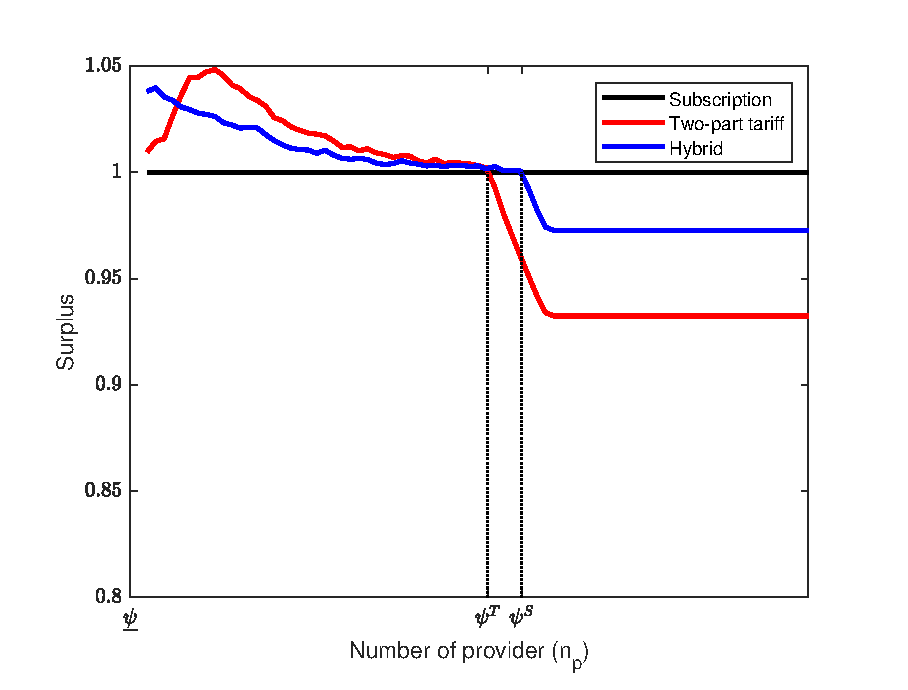
\includegraphics[width=5cm]{figure_3rd_final/prop_c_6_1.eps}}    
    \caption{Numerical Analysis on Heterogeneous Storage Volume (Utility Function I, Scenario ii)}
\end{figure}
%- 아래의 pareto distribution에서 parameter가 달라질 때 효과와 연결\\
%- 용량이 큰 고객의 $b$가 큰 경우에, 이들에게는 i) first-best 인 부분에서 bandwidth에 비용을 지불받는 것의 merit이 줄어들어 subscription과 가까워짐 2) 마찬가지로 market-clearing에서도 bandwidth로부터 얻는 이익이 많이 없어져서 subscription과 가까워짐 -- c로 갈 수록 전체적으로 subscription과 가까워지는 모습(특히, hybrid)\\

\newpage

\textbf{Utility function II.}  When the bandwidth allowance is constant\\
\underline{\textit{Scenario i})} $(b_l, b_h) = (2, 2)$
\begin{figure}[ht!]
\def\figurename{Figure R2 -}
    \centering
    \subfigure[$Low:High = 9:1$]{\includegraphics[width=5cm]{figure_3rd_final/volume_c_1.eps}}
    \subfigure[$Low:High = 5:5$]{\includegraphics[width=5cm]{figure_3rd_final/volume_c_2.eps}}
    \subfigure[$Low:High = 1:9$]{\includegraphics[width=5cm]{figure_3rd_final/volume_c_3.eps}}
    \caption{Numerical Analysis on Heterogeneous Storage Volume (Utility Function II, Scenario i)}
\end{figure}

\underline{\textit{Scenario ii})} $(b_l, b_h) = (2, 5)$
%%%%%%%%%%%%%%%%%%
\begin{figure}[ht!]
\def\figurename{Figure R2 -}
    \centering
    \subfigure[$Low:High = 9:1$]{\includegraphics[width=5cm]{figure_3rd_final/volume_c_4.eps}}
    \subfigure[$Low:High = 5:5$]{\includegraphics[width=5cm]{figure_3rd_final/volume_c_5.eps}}
    \subfigure[$Low:High = 1:9$]{\includegraphics[width=5cm]{figure_3rd_final/volume_c_6.eps}}
    \caption{Numerical Analysis on Heterogeneous Storage Volume (Utility Function II, Scenario ii)}
\end{figure}

\begin{quotation}
{\em
\noindent \textbf{Reviewer 2 (Point A2b): }
b. Compared to the concern on the unit volume of each renter, perhaps the assumption that each provider supplies unit volume of unused capacity is fine. But the implication is that the provider’s income and cost are both proportional to the volume of capacity supplied. If this is most likely the case in the storage sharing industry, the authors need to explain this point to justify this assumption; otherwise, I wonder whether the authors could relax this assumption, i.e., whether the impacts of a specific pricing scheme on providers with different capacity are different.}
\end{quotation}\vspace{-4mm}

This is another great point. As you indicated, we can safely ensure the validity of our findings if each provider's income and cost are both proportional to his storage capacity. Specifically, we set each provider's operating cost to be proportional to $\hat{\omega_b}$ (i.e., the expected bandwidth volume for each provider), and $\hat{\omega_b}$ is proportional to each provider's shared storage capacity. Below, we discuss whether this assumption is consistent with the reality, and potential implications of alternative cost forms.

\textbf{Is the operating cost proportional to $\hat{\omega_b}$?} The operating costs may include various sources, such as Internet bandwidth, electricity costs, and obsolescence of the computing device. Intuitively, bandwidth and electricity costs are proportional to bandwidth usage. Hardware obsolescence is directly related to the computational burden, and it is attributable to both computation amount and running time. Although the exact functional form of this relationship is unknown, its impact tends to be secondary to other direct costs (i.e., bandwidth and electricity) and is partially absorbed by $\xi(t)$. Thus, it is plausible to assume that the operating cost is proportional to $\hat{\omega_b}$.

\textbf{Is $\hat{\omega_b}$ proportional to the provider's capacity?} P2P storage platforms usually encourage providers to share more capacity by mentioning that sharing more capacity will lead to more access from renters and more earnings. Also, it is commonly observed that providers with higher capacity tend to store more files than those with lower capacity on these platforms. Thus, it is plausible to assume that the platform assigns more files and bandwidth services to high-capacity providers than low-capacity ones.

\textbf{How would alternative cost forms affect the results?} Alternative cost functions may affect our main insights as follows. First, we may consider a convex function, such as quadratic and exponential forms, where operating costs are particularly burdensome for high-capacity providers. In this case, as high-capacity providers bear much higher operating costs and join the platform less, the first-best prices will be less achievable. Hence, compensating for offering bandwidth services will have a higher impact on the storage capacity. Consequently, the relative benefits of two-part tariff and hybrid pricing (vs. subscription-based pricing), which mainly come from enhancing the platform's capacity, will be greater in this situation.

Second, we may also consider a concave function of operating costs like a square root function. Since high-capacity providers bear relatively less operating burden than they do in the current setup, the platform will attract more providers under the subscription-based pricing---which does not compensate for offering bandwidth services. Therefore, the profit/surplus gap between the subscription and other pricing schemes will decrease as a result. However, although the magnitudes decline, we expect the differences to remain qualitatively unchanged.

We have summarized this discussion in the revised manuscript as follows:

``Second, one might consider an alternative form of the provider's operating cost. Basically, the current form relies on the assumptions that operating costs are proportional to $\hat{\omega_b}$ (i.e., the expected bandwidth volume for each provider), and that $\hat{\omega_b}$ is proportional to each provider's shared storage capacity. We argue that these assumptions are plausible for the following reasons: 1) many of the major costs, such as Internet bandwidth and electricity costs, are proportional to bandwidth usage, and 2) the platform tends to assign more files and bandwidth services to high-capacity providers than low-capacity ones.

So, how would alternative cost forms affect the results? On the one hand, we may consider a convex function, such as quadratic and exponential forms, where operating costs are particularly burdensome for high-capacity providers. In this case, as high-capacity providers bear much higher operating costs and join the platform less, compensating for offering bandwidth services will have a higher impact on the storage capacity. Consequently, the relative benefits of two-part tariff and hybrid pricing (vs. subscription-based pricing) will be greater in this situation. On the other hand, we may also consider a concave function like a square root function. Since high-capacity providers bear relatively less operating burden than they do in the current setup, the platform will attract more providers under the subscription-based pricing. Hence, the profit/surplus gap between the subscription and other pricing schemes will decrease as a result. However, although the magnitudes decline, we expect the differences to remain qualitatively unchanged.'' (page 31)

\begin{quotation}
{\em
\noindent \textbf{Reviewer 2 (Point A3):  }3. A provider’s decision is based on his knowledge of the expected demand for the storage service and the bandwidth service, which, however, are dependent on conditions of the whole market. In practice, how can an individual provider possess such information? Does the platform facilitate information sharing?}
\end{quotation}\vspace{-4mm}

P2P storage providers have multiple sources that offer information before joining the platform.\footnote{Some examples of information sources:
\begin{itemize}
    \item SiaStats: \url{https://siastats.info/}
    \item Reddit community for Sia \url{https://www.reddit.com/r/siacoin/}
    \item Storj's prerequisites: \url{https://docs.storj.io/node/before-you-begin/prerequisites/}
    \item Filefox (a Filecoin blockchain explorer): \url{https://filfox.info/en/}.
\end{itemize}} For example, SiaStats is a website that publicizes Sia's storage sharing status, such as used storage, number of transactions, network revenues, and hash rates. Also, individual providers have actively analyzed and shared their profitability in online forums like Reddit. Moreover, the P2P platforms notice the minimum requirement and recommended capacity of computing resources before individual providers decide to participate in their networks. Such information can partially inform them about their expected operational costs.

After joining the platform, providers can receive real-time feedback on their network performance; thus, they can quickly correct their behaviors on the platform. Even when unsuccessful on the platform, they can quickly leave the network similarly to other digital markets. Thanks to the platform-offered information, online forums, and easiness of market entry/exit, we expect that P2P participants will reach market equilibrium very rapidly. We have described this background in the new version as follows:

``Third, and importantly, one might wonder if providers can meaningfully predict the demand for storage and bandwidth services in advance. We argue that providers can make informed choices based on multiple sources that offer information before joining the platform. For example, individual providers have actively analyzed and shared their profitability in online forums, such as Reddit. Also, the P2P storage platforms notice their minimum requirement and recommended capacity of computing resources before individuals decide to join their networks. Such information can partially inform them about their expected operational costs. They also publicize their storage sharing status, such as used storage, number of transactions, network revenues, and hash rates (e.g., SiaStats). Moreover, even when unsuccessful on the platform, they can quickly leave the network, similar to other digital markets. In sum, due to the platform-offered information, online forums, and easiness of market entry/exit, we expect that participants in the platform will rapidly reach market equilibrium.'' (pages 31-32)

\begin{quotation}
{\em
\noindent \textbf{Reviewer 2 (Point A4a):  }4. Other model assumptions to justify: a. The assumption about independence of a renter’s utility from the download bandwidth service from her download frequency is questionable. One may argue that the two parameters are positively correlated as the more frequent the renter needs to access the storage, the more valuable the bandwidth service means to her.}
\end{quotation}\vspace{-4mm}

This is another great point. In our analysis, we have postulated that a renter's utility per bandwidth volume is independent of her download frequency. Let us note that among renters adopting the platform, the utility per volume and the download frequency are already positively associated with each other as a result of self-selection. In this regard, if the two parameters are positively correlated among all potential renters, we will obtain a more dramatic relationship among platform-adopting renters. Therefore, we expect that the implications of pricing schemes will be qualitatively consistent.

We have validated this conjecture by examining a scenario where potential renters with the higher utility per download volume tend to have more frequent download requests. We have manipulated the shape parameter $b$ of the Pareto distribution---which determines the extent to which the bandwidth frequency is concentrated or dispersed---differently by the utility per bandwidth volume. Specifically, we have divided potential renters into two groups: 1) renters whose unit utility is uniformly distributed in $[0, 0.5]$ and whose frequency follows the Pareto distribution having a lighter tail (with $b_l=5$), and 2) those whose unit utility is uniformly distributed in $[0.5, 1]$ and whose frequency follows the Pareto distribution having a heavier tail (with $b_h=2$), where $b_l > b_h$. For this scenario, we have conducted a numerical analysis and obtained qualitatively similar results (see \textbf{Figure R2-5}).

\begin{figure}[ht!]
\def\figurename{Figure R2 -}
\centering
\includegraphics[width=8cm]{figure_3rd_final/half_1.eps} 
\caption{Numerical Analysis on Positive Association Between Utility per Download and Download Frequency. The red (blue) line indicates the relative total surplus of the two-part tariff (the hybrid pricing) compared with the subscription-based pricing, which is represented as the horizontal black line.}
\end{figure}

The revised manuscript provides a summary of this discussion as below :

``Also, our model postulates that the distributions of the utility per bandwidth volume and the download frequency are independent. Although this leads to a positive association between these variables as a result of self-selection, it is also possible that they are positively associated with each other before the renter's decision. We examine whether the implications of pricing schemes are qualitatively consistent after relaxing this assumption by conducting a numerical study. We observe that our main findings remain qualitatively consistent.'' (page 32)

\begin{quotation}
{\em
\noindent \textbf{Reviewer 2 (Point A4b):  }b. The assumption that the renters’ bandwidth usage level follows a Pareto distribution needs better justification. Are there other studies (or empirical evidence) than Li and Kumar (2018) that also adopt this assumption? Can the same results be derived based on other distributions (e.g., Poisson)?}
\end{quotation}\vspace{-4mm}

We apologize that we did not sufficiently justify our using a Pareto distribution. In adherence to your comments, we have added prior studies that adopted this assumption and examined whether our results are restricted to the heavy tail distribution in this revision.

In our description of the related literature, we have supplemented prior studies that utilized the Pareto distribution following the empirical findings of Loboz (2012). Moreover, we have provided additional examples showing that digital consumption is likely to have heavy-tailed distributions. The following presents our revised paragraph:

``This model concerns renters with a continuum of bandwidth usage level (or frequency of download requests) of stored files denoted by $\lambda$. It has been empirically observed in the literature that the usage of cloud-resource is distributed with relatively heavy tails compared with exponential, log-normal, and normal distributions (Loboz, 2012), similarly to other digital resources like smartphone and YouTube usage (Falaki et al., 2010; Gill et al., 2008). Thus, we assume that a renter’s bandwidth usage $\lambda$ follows the Pareto distribution in keeping with the extant literature (Bandi et al., 2015; Li and Kumar, 2018; Ramírez-Velarde et al., 2017).'' (page 12)

%시나리오 1. pareto 밖에 안될 경우 -> 우리가 renter의 frequency 분포가 달라지는 경우들을 여러가지로 고려해보기 위하여, 기존의 shape parameter와 다른 b 값을 넣어서 테스트를 해보았다. (이 경우에는 b값에 따라 달라지는 pareto distribution을 그래프 혹은 표로 + 정보로 넣는것도 방법일듯?) 그럼에도 불구하고 똑같았다. 

%시나리오 2. 다 될 경우 -> 다 해봤다. 똑같았다.

Although the heavy-tail assumption has been empirically confirmed, the exact shape might vary across contexts and affect the results differently. To assess whether our results are restricted to the current parameter, we have conducted a numerical analysis for different shapes of distributional tails. We have varied the Pareto's shape parameters and tested whether our findings hold. The results in \textbf{Figure R2-6}) suggest that, in line with the insights from our closed-form results, the total surplus of the two-part tariff and the hybrid pricing can be higher (lower) than the subscription-based pricing when the number of potential providers is small (large).

% \begin{figure}[ht!]
% \centering
% \includegraphics[width=8cm]{figure_3rd_final/f_main_modify.eps} 
% \caption{main}
% \end{figure}
%%%%%%%%%%%%%%%%%%%%%%%
\begin{figure}[ht!]
\def\figurename{Figure R2 -}
    \centering
    \subfigure[$b = 3$]{\includegraphics[width=5cm]{figure_3rd_final/main_3.eps}}
    \subfigure[$b=4$]{\includegraphics[width=5cm]{figure_3rd_final/main_4.eps}}
    \subfigure[$b=5$]{\includegraphics[width=5cm]{figure_3rd_final/main_5.eps}}    
    \caption{Numerical Analysis on Different Parameters of the Pareto Distribution. The red (blue) line indicates the relative total surplus of the two-part tariff (the hybrid pricing) compared with the subscription-based pricing, which is represented as the horizontal black line.}
\end{figure}
%%%%%%%%%%%%%%%%%%%%%%%
% 그래프 설명:\\
% $b$가 커짐에 따라서 two-part tariff, hybrid가 subscription에 가까워짐. \\
% $b$가 커진다는 것은 높은 사용량을 가지는 renter들의 비중이 적다는 뜻. \\
% 따라서 이 경우에 발생하는 현상은 두 가지 dimension으로 설명 가능.\\
% i) bandwidth에 대하여 비용을 부과하는 방식에는 당연히 사용량이 많은 renter들이 더 큰 영향을 받음. 따라서, 사용량이 많은 고객이 적어질 수록, bandwidth price 부과로 인하여 surplus가 감소하는 고객들도 줄어듬. 이로 인해 first-best 범위 내에서도 surplus 발생하는 차이가 줄어들게 됌.\\

% bandwidth에 비용을 부과하는 hybrid, two-part tariff를 통하여 provider에게 충분한 보상이 제공되어, provider을 확보하는데 도움이 되는 logic 자체는 bandwidth를 많이 사용하는 renter들이 많아서 pricing scheme을 변경함으로써 provider에게 더 많은 보상을 제공할 수 있을 때 극대화되는 효과. 따라서, $b$가 커져서 bandwidth를 많이 사용하는 고객들이 줄어드는 상황에서는 hybrid 및 two-part tariff가

We have discussed this point in the new version as follows:

``First, we find that our findings remain consistent when we relax the assumption of bandwidth usage distribution. 
Specifically, we assume that bandwidth usage follows the Pareto distribution with $b=2$ to account for the heavy-tail distribution and analytical tractability. To assess whether this assumption is entirely responsible for our findings, we conduct a numerical analysis of different shapes of distributional tails. For ease of comparison, we have varied the Pareto’s shape parameters and tested whether our findings hold. The results show that the implications of pricing schemes do not change under different parametric conditions.'' (page 32)

\textbf{References}

Bandi, C., Bertsimas, D., & Youssef, N. 2015. Robust Queueing Theory. \textit{Operations Research}, 63(3), 676-700.

Falaki, H., R. Mahajan, S. Kandula, D. Lymberopoulos, R. Govindan, D. Estrin. 2010. Diversity in smartphone usage. S. Banerjee, ed. \textit{Proceedings of the 8th International Conference on Mobile Systems, Applications, and Services}. ACM, New York, NY, 179–194.

Gill, P., M. Arlitt, Z. Li, A. Mahanti. 2008. Characterizing user sessions on youtube. R. Rejaie, R. Zimmermann, eds. \textit{Electronic Imaging} 2008. International Society for Optics and Photonics, Bellingham, WA, 681806–681814.

Li B, Kumar S (2018) Should you kill or embrace your competitor: Cloud service and competition
strategy. \textit{Production and Operations Management} 27(5):822–838.

Loboz C (2012) Cloud resource usage—heavy tailed distributions invalidating traditional capacity planning models. \textit{Journal of Grid Computing} 10(1):85–108.

Ramírez-Velarde, R., Tchernykh, A., Barba-Jimenez, C., Hirales-Carbajal, A., Nolazco-Flores, J. 2017. Adaptive Resource Allocation with Job Runtime Uncertainty. \textit{Journal of Grid Computing}, 15(4), 415-434.

%%%%%%%%%%%%%%%%%%%%%%%%%%%%%%%%%%%%%%%%%%%%%%%%%%%%%%%%%%%%%%%%%%%%%%%%%
\noindent\textbf{Suggestions on writing of some subsections:}\\[-11mm]
%%%%%%%%%%%%%%%%%%%%%%%%%%%%%%%%%%%%%%%%%%%%%%%%%%%%%%%%%%%%%%%%%%%%%%%%%
\begin{quotation}
{\em
\noindent \textbf{Reviewer 2 (Point B1):  }1. In subsection 3.2, the presentation of the provider’s profit function is somewhat unclear. The reader may wonder how to derive the expected storage and bandwidth volume for each provider ($\hat{\omega}_s, \hat{\omega}_b$, and $\hat{\omega}_{bp}$), while it turns out that the derivations will be introduced later in section 4. Moreover, to facilitate the reader’s understanding of the formulation, it would be better to explain why $\hat{\omega}_b = \hat{\omega}_s \cdot \nu_b / (\theta \nu_s)$ holds (i.e., the meaning of the ratio $\nu_b / (\theta \nu_s) $is not immediately clear to the reader). }
\end{quotation}\vspace{-4mm}

Thank you for these constructive comments on describing our model setup. First, we agree that the necessary information needed to understand the provider's decision in Section 3.2---the notations for the expected storage and bandwidth volume, shaped by renters' aggregate decisions---appeared too late in the last version. To address this point, we have moved the renter's decisions and relevant notations from Section 4 to the beginning of Section 3.2. We believe that this restructuring will substantially help improve the readability of our paper.

Second, we have further elaborated the meaning of $\hat{\omega}_b = \hat{\omega}_s \cdot \nu_b / (\theta \nu_s)$, which was used to describe the provider's profit function $\pi_j =\alpha (\hat{\omega}_s p_s + \hat{\omega}_{bp} p_b) - \rho_j \hat{\omega}_b \xi$. In the new version, we have revised this equation to better present that the platform randomly assigns storage demand to participating providers. 

Specifically, we have replaced the equation from
\begin{equation*}
	\hat{\omega}_b = \hat{\omega}_s \cdot \frac{\upsilon_b}{\theta \upsilon_s} 
\end{equation*}
to
\begin{equation*}
	\hat \omega_b = \frac{\hat \omega_s}{\theta \upsilon_s} \cdot \upsilon_b.
\end{equation*}
Here, $\hat \omega_s$ is the individual provider's expected storage volume, and $\theta \upsilon_s$ indicates the total storage demand multiplied by the redundancy rate in the network. Therefore, $\hat \omega_s / (\theta \upsilon_s)$ implies that the platform assigns bandwidth volume to each provider proportionally to his share from the entire stored volume. In other words, each provider obtains a smaller portion of the storage and bandwidth volumes as more providers join the platform.

\begin{quotation}
{\em
\noindent \textbf{Reviewer 2 (Point B1a):  }a. Similarly, it would be better to explain, for the platform’s decision problem, why $V_{bp} = V_s \cdot \nu_{bp} / (\theta \nu_s)$ (i.e., the meaning of the ratio $\nu_{bp} / (\theta \nu_s) $ is not immediately clear to the reader).}
\end{quotation}\vspace{-4mm}

In the new version, we have provided the platform's optimization problem in Section 4. In the equation $V_{bp} = V_s \cdot \nu_{bp} / (\theta \nu_s)$ of this problem, $V_s = \min\{\theta \upsilon_s, \omega_s\}$ is the total volume of shared storage, and $V_s / (\theta \nu_s)$ means the share of stored data from the total storage demand. We have added this interpretation and explained why we can reduce this constraint into $\theta \upsilon_s \le \omega_s$ as follows:

``Here, $V_s$ is the total volume of shared storage and $V_s / (\theta \upsilon_s)$ means the share of stored data from the total storage demand. When there are sufficient participating providers, $V_s = \theta \upsilon_s$ and $V_{bp} = \upsilon_{bp}$. Otherwise, $V_s = \omega_s$ and $V_{bp} = (\omega_s / \theta \upsilon_s) \cdot \upsilon_{bp} < \upsilon_{bp}$, indicating that the total paid bandwidth volume is smaller than the bandwidth demand.

Importantly, in the second scenario (i.e., $V_s = \omega_s$), the platform can always increase its profit by raising service fees. This is because the platform can attract a larger number of providers and serve more storage volume. For this reason, we can reduce this platform's problem into the equivalent problem as follows:'' (pages 19-20)

\begin{quotation}
{\em
\noindent \textbf{Reviewer 2 (Point B1b):  }b. On a related note, in the formulation of the providers’ total surplus PS (at the end of page 20), it seems that the authors assume $\rho_j$ is uniformly distributed over $[0,1]$, but I didn’t find the statement of this assumption (or perhaps I just missed it).}
\end{quotation}\vspace{-4mm}

Thank you for this comment. Yes, $\rho_j$ is uniformly distributed over $[0,1]$ as you noted. After reviewing our previous manuscript, we have found that our explanation of this assumption was difficult for readers to notice. Therefore, we have revised Section 3.1 to make this assumption more salient. In addition, we have restated this when we have mentioned that $\rho_j$ is heterogeneous in Section 3.2.2.

\begin{quotation}
{\em
\noindent \textbf{Reviewer 2 (Point B2):  }2. The literature review needs to be streamlined. For example, on top of page 7, the discussion is about “this study also extends the literature on sharing platforms for computing resources,” then, on the same page, the discussion continues to be about “emerging platforms have enabled sharing various computing resources.” But, later on page 8, again the discussion goes back to “this study also contributes to the literature on the pricing for resource sharing services.” The writing of these paragraphs feels like on an ad hoc basis. Maybe a better sequence is as follows: (1) pricing (and capacity management) in centralized public cloud; (2) P2P sharing of computing resources; (3) literature on other forms of sharing economies. Finally, in the last paragraph, summarize the distinct model features and contribution to the existing literature.}
\end{quotation}\vspace{-4mm}

Thank you for these constructive comments on our literature review. In keeping with your suggestions, we have reorganized this section as follows. Please also note that for readability, we have separated our contributions from these subsections and made a separate subsection, Section 2.4.

\begin{center}
\textbf{2.1 Pricing and Capacity Management in Centralized Cloud}
$$\Downarrow$$
\textbf{2.2 P2P Sharing of Computing Resources}
$$\Downarrow$$
\textbf{2.3 Sharing Economy and Online Platforms}
$$\Downarrow$$
\textbf{2.4 Contributions to the Literature}
\end{center}

We sincerely appreciate your suggestions, which helped us better streamline our literature review and clarify our contributions.

\end{document} 
